%! Author = stefano
%! Date = 22/11/2020

% Preamble
\documentclass[11pt]{article}
\usepackage[utf8]{inputenc}
\usepackage{dirtree}
\usepackage{graphicx}
\graphicspath{ {../images/} }
\usepackage[margin=1in]{geometry}


\title{Pedestrian Intent Prediction}
\author{Stefano Zanatta, Pasquale Coscia, Lamberto Ballan}
\date{\today}

% Packages
\usepackage{apacite}
\usepackage{amsmath}
\usepackage{hyperref}
\usepackage{biblatex}

% Document
\begin{document}
\maketitle


\section{Introduction}
    We implemented the work of Haziq Razali, Alexandre Alah:
    Pedestrian-Intention-Prediction\cite{PedestrianIP}.
    The original work consists in a Convolutional Neural Network - LSTM, with the goal to predict the intention
    of pedestrians on crossing the road.\\
    The model was originally trained on Lausanne Dataset (not public) and on JAAD Dataset\footnote{\url{http://data.nvision2.eecs.yorku.ca/JAAD_dataset/}}.
    The former was recorded by static cameras, the latter on moving cameras (placed in the cars).\\
    The goal of this project is to study the pipeline, reproduce the experiments, adapt and
    improve the model for the JAAD and PIE datasets\footnote{\url{https://data.nvision2.eecs.yorku.ca/PIE_dataset/}}.

\section{Lausanne Dataset}
    %TODO general results on lausanne (by Haziq Razali)

\section{JAAD Dataset}
    The JAAD datasets consists of mp4 videos, each one associated to a rich description, frame to frame, of what is happening on a given moment:
    \begin{itemize}
        \item id of the pedestrian
        \item coordinates of the pedestrian on the relative frame
        \item standing, walking
        \item looking at the traffic
        \item hand gesture
        \item speeding up/slowing down
        \item crossing the road
        \item occlusion
    \end{itemize}
    For the target we only use the information about crossing the road.\\
    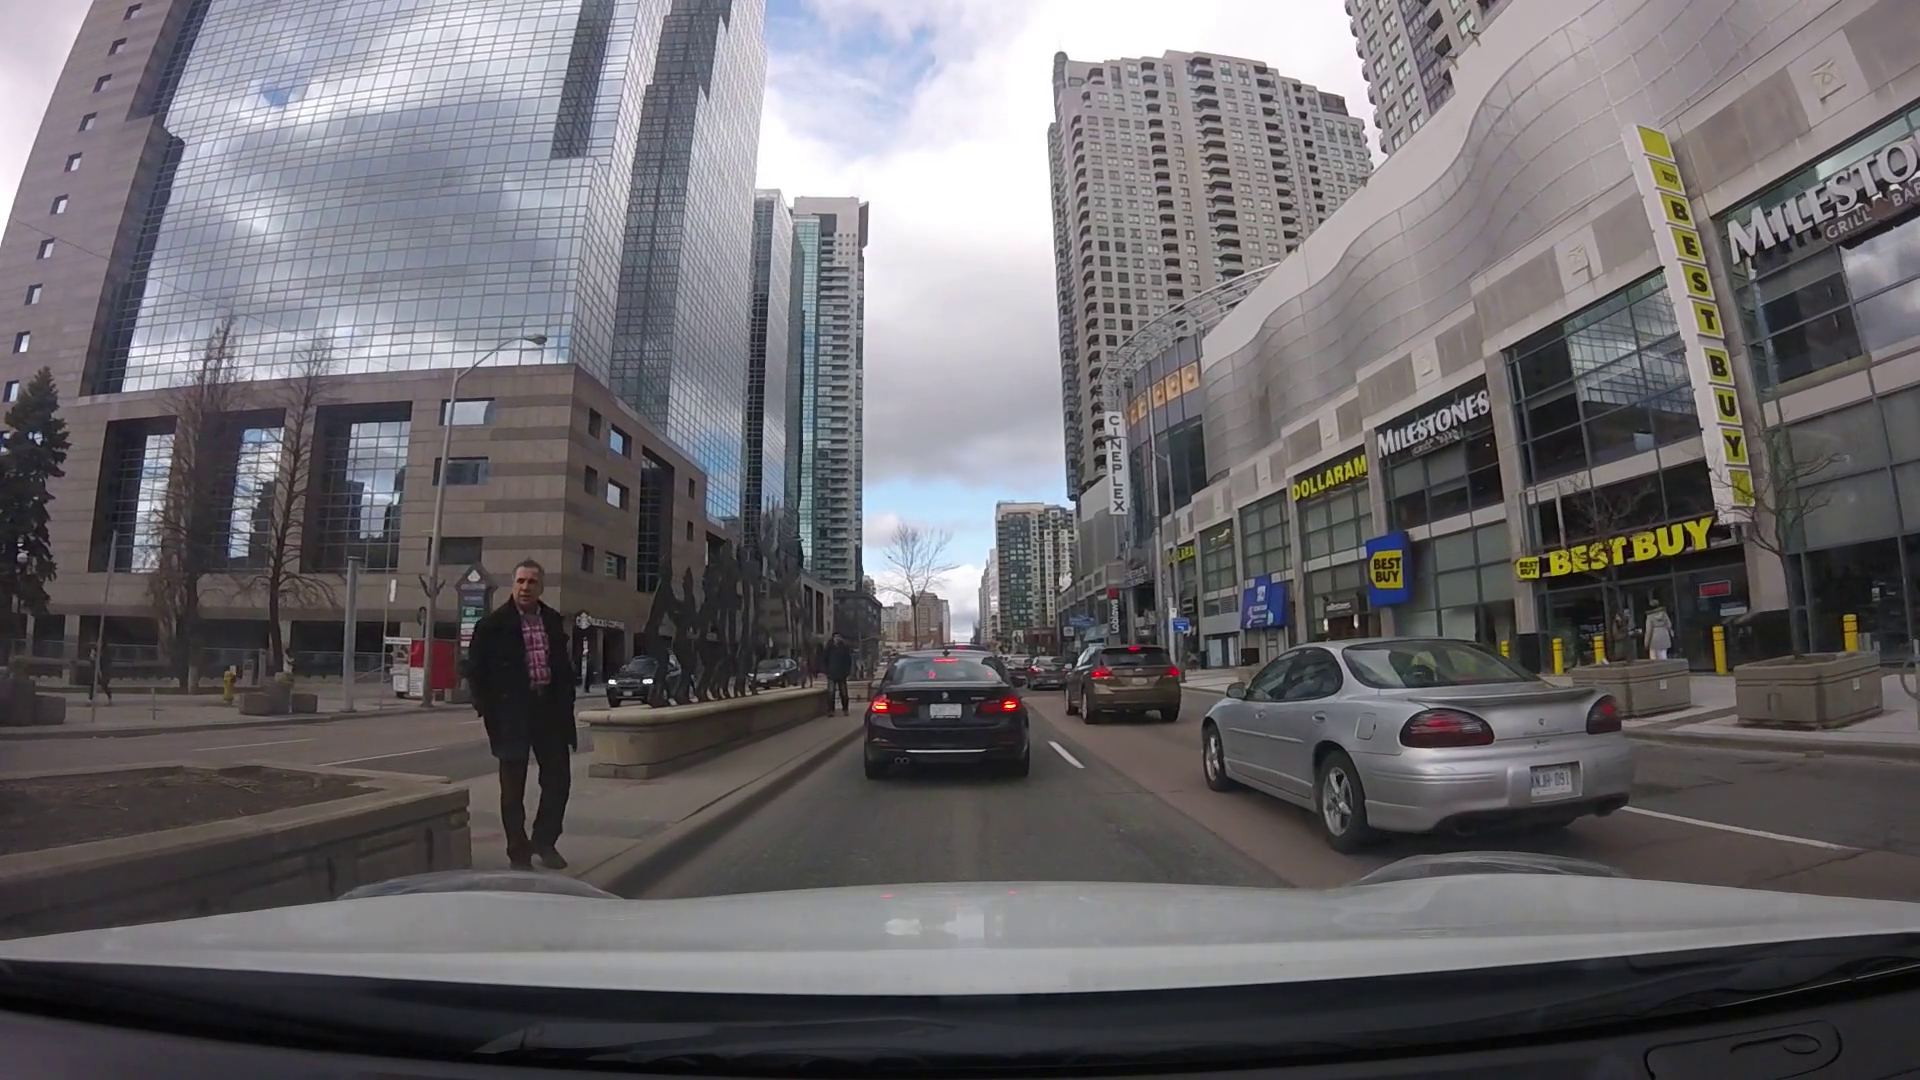
\includegraphics[width=\textwidth]{jaadscene}\\

\section{Pipeline}
\subsection*{Adapting the ground truth}
    The first step is to create the ground truth for the model by transforming the input into a csv.
    Originally, the Lausanne dataset required a step to locate the pedestrians (with an external object detector)
    and the (static) coordinates of the road.
    This is not longer required, because JAAD and PIE include the coordinates of the pedestrians and whether or not
    they are crossing the road.
    \begin{center}
    \begin{tabular}{ c c c c c c c c c c}
     frame & id & tlx & tly & width & height & walking & standing & looking & incrossing\\
     1,0 & 463 & 730 & 69 & 118 & 0 & 1 & 0 & 0 & 0\\
     1,0 & 463 & 730 & 69 & 118 & 0 & 1 & 0 & 0 & 1\\
    \end{tabular}
    \end{center}
\subsection*{Trajectories}
    The second Step consists in assigning, at each frame, the ``lifetime'' of the pedestrian in the video, and a ``cross'' column, indicating if they
    ever crossed the road in their lifetime.
    \begin{center}
    \begin{tabular}{ c c c}
     incrossing & lifetime & cross\\
     0 & 568 & 0\\
     0 & 568 & 0\\
    \end{tabular}
    \end{center}

\subsection*{Hungarian Tracker}
    Remove pedestrians with a lifetime below a threshold, and change pedestrians IDs to a numeric value.
    We had to change the algorithm that defined whether the pedestrian crossed or not the road, before it was designed for
    videos where the pedestrian always started from a (non-crossing) side of the screen and then, eventually, he could cross the road
    or not.
    Now the new algorithm does not make any assumption on the initial position, to adapt to the JAAD and PIE datasets, where
    pedestrians can alternate the crossing of the road with the non-crossing and start in a crossing position.
    For example, this is the first frame of the Jaad video n\°5. In this case we expect the model to predict ``will cross''
    for each pedestrian in the screen.\\
    \includegraphics[width=0.5\textwidth]{crossing0}\\
\subsection*{Crop Pedestrians}
    Crops each pedestrian into images, organized in sub-folders:
    \dirtree{%
        .1 dataset.
        .2 all.
        .3 crops.
        .4 name\_of\_the\_video.
        .5 id\_of\_the\_pedestrian.
        .6 id\_pedestrian\_png.
    }\\
    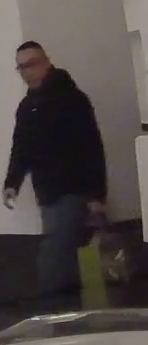
\includegraphics[width=0.2\textwidth]{crop}\\
    Then appends the path of the crop to each frame's annotation.
    \begin{center}
    \begin{tabular}{ c c c c c c c c c c c c c c}
     filename & folderpath\\
     00000001.png & crops\video\_0001\0000000000\\
     00000001.png & crops\video\_0001\0000000000\\
    \end{tabular}
    \end{center}
\subsection*{Save Scenes}
    Add the whole scenes to the dataset and adds their paths to the annotations.
    \dirtree{%
        .1 dataset.
        .2 all.
        .3 scenes.
        .4 name\_of\_the\_video.
        .5 id\_video\_png.
    }
    The new annotations columns are:
    \begin{center}
    \begin{tabular}{ c c }
     scene\_filename & scene\_folderpath \\
     00000001.png & scenes\video\_0001 \\
     00000001.png & scenes\video\_0001 \\
    \end{tabular}
    \end{center}

\subsection*{Split train test}
    In the last step the dataset is split into train and test:
    \dirtree{%
    .1 dataset.
    .2 train.
    }\\
    \dirtree{%
    .1 dataset.
    .2 test.
    }
\section{Model}
The model is composed of a VGG-16 pre trained CNN, a fully connected layer (feature embedder), a LSTM and
a linear classifier to predict if the pedestrian crossed the road.
Unless differently specified, we used 50 epochs, sequences of 8 observed frames for each prediction (obs\_len), 32 batch size.\\
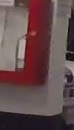
\includegraphics[width=0.25\textwidth]{jaaderrorcrop}\\

\subsection*{VGG-16}
VGG-16 is a (pre-trained CNN) feature extractor.
This operation is executed for each image in the batch.
\subsection*{Feature Embedder}
Embed the CNN output into a 255 units vector.
Then performs dropout (0.5).

\subsection*{LSTM}
Process the sequence through the LSTM with ReLU activation function and dropout.


\subsection*{Linear Classifier}
Classify whether the pedestrian crossed the road or not.

\subsection*{Changes to the original model}
To improve the results, we added the entire scene as input for the prediction (JAADScene).
We added a new VGG-16 CNN, followed by a LSTM to create the sequence, then we merged the scene-LSTM output with the crops-LSTM
outputs and adapted the input size of the linear predictor. (\#todo) % todo

\\
For another version of the model, we added more actions as target for the linear predictor.
This makes the task harder, but should make the model more robust to overfitting.(\#todo) %TODO


\section{PIE Dataset}
\#todo

\section{PIE Pipeline}
\#todo


\section{Results}
    The model works best when there is a clear distinction between the pedestrians are not-crossing (for their initial lifetime)
    and crossing the road (at the end of their lifetime).
    It works poorly for large roads where the same pedestrians can move in and out the road repeatedly.\\
    The original experiments where done on datasets where the direction of movement of the pedestrians where already known.
    For the Jaad dataset the directions were unknown and the results were much worse.\\
    \includegraphics[width=\textwidth]{results_original}\\
    To get better results we had to remove the draw-trajectories min-lifetime thresholds (so a pedestrian is considered more often, even if they are
    crossing the road at frame 0 and leaves the screen shortly after).
    This change improved the results by increasing the dataset size.\\
    The following results show the base model trained on Jaad dataset and the model improved with the scenes input.\\
    (all results are based on test data).

    \begin{center}
    \begin{tabular}{| c c c c |}\hline
     Model & Precision & Recall & Accuracy\\
     Jaad & 0.750 & 0.558 & 0.6714285714285714 \\
     Jaad+Scenes & 0.742 & 0.535 & 0.7428571428571429\\\hline
    \end{tabular}
    \end{center}

    The results improved by adding the scenes, but the train accuracy (0.977) is still much higher, showing some overfitting.



\section{Changes to the Model}
We tested some changes to the hyperparameters or the structure of the baseline model.
We started by changing the feature extractor (pretrained CNNs) and then implementing ideas from different works on JAAD.

\subsection*{Changing the pre-trained CNNs}
We tested the same model changing the pretrained VGG-16 CNN (just with crops).
Googlenet (best CNN for crops) scenes resulted in worse accuracy when applied to the scenes.


\begin{center}
\begin{tabular}{| c c c c |}\hline
    Model           & Precision & Recall & Accuracy\\
    VGG-16 CNN      & 0.750     & 0.558  & 0.6714285714285714 \\
    Wide Resnet50 2 & 0.622     & 0.535  & 0.6571428571428571 \\
    googlenet       & 0.733     & 0.512  & 0.6857142857142857 \\
    densenet201     & 0.565     & 0.302  & 0.6428571428571429 \\
    googlenet+scenes &  0.600  &  0.188     &  0.7 \\              \hline



\end{tabular}
\end{center}

We explored some works tested on the JAAD dataset by different authors.
\subsection*{Spatiotemporal Relationship Reasoning for Pedestrian Intent Prediction}
They\cite{liu2020spatiotemporal} based their network on
Graph Convolutional Neural Networks\cite{GCNN}, by viewing the scene as a graph and then applying the same convolutions
to different zones.
The prediction accuracy was at its best at 30 frames (1 second), dropping by \textasciitilde 10\% after the 90\textsuperscript{th} and
before the 10\textsuperscript{th} frame.
In our work we predicted the next move after 8 frames, so we increased that to 30 for a comparison.
The accuracy did not improve and the training times increased by too much, so we did not try the 60 and 90 frames prediction.

\begin{center}
\begin{tabular}{| c c c |}\hline
    model & frames & Accuracy on K\textsuperscript{th} frame\\
    Graph-CNN & 30 & 0.7698 \\
    Graph-CNN & 60 & 0.7309 \\
    Graph-CNN & 90 & 0.6831 \\
    Crops+googlenet(ours) & 30 & 0.578947368421053 \\\hline

\end{tabular}
\end{center}

\subsection*{PEDESTRIAN INTENTION PREDICTION: A MULTI-TASK PERSPECTIVE}
This model is more similar to ours, because it inputs the pedestrian's cropped images to a feature extractor (CNN), a
LSTM and to a fully connected layer for prediction.
Hyperparameters set to 100 (instead of 50) epochs and 12 frames per sequence (instead of 8).
The main difference is that they perform multi-tasking learning, predicting both the crossing/non-crossing and the velocity of
each bounding box (for each pedestrian).
They also tested the same model adding the scene to the input (other then the crops), but reducing their size for faster training.\\
Adding a different task (velocity prediction) improved the intent prediction by \textasciitilde 2\%.

\begin{center}
\begin{tabular}{| c c |}\hline
    model & Accuracy\\

    Single-task PV-LSTM & 08967\\
    Multi-task PV-LSTM & 0.9148\\\hline

\end{tabular}
\end{center}
We implemented the multitask learning approach, but could not compare the results because we did not have access to the
velocity for the bounding boxes.

\begin{center}
\begin{tabular}{| c c c c |}\hline
    model & precision & recall & Accuracy\\
    googlenet+scenes &  0.600  &  0.188 &  0.7 \\


\end{tabular}
\end{center}



\bibliographystyle{apacite}  % works with overleaf
\bibliography{mainbib}

\end{document}


scenes with 30 frames prediction
[INFO: train.py:  234]:   [val] d_accuracy: 0.605
[INFO: train.py:  234]:   [val] d_fn: 13.000
[INFO: train.py:  234]:   [val] d_fp: 2.000
[INFO: train.py:  234]:   [val] d_loss: 0.847
[INFO: train.py:  234]:   [val] d_precision: 0.600
[INFO: train.py:  234]:   [val] d_recall: 0.188
[INFO: train.py:  234]:   [val] d_tn: 20.000
[INFO: train.py:  234]:   [val] d_tp: 3.000
[INFO: train.py:  237]:   [train] d_accuracy: 0.686
[INFO: train.py:  237]:   [train] d_fn: 42.000
[INFO: train.py:  237]:   [train] d_fp: 22.000
[INFO: train.py:  237]:   [train] d_loss: 0.658
[INFO: train.py:  237]:   [train] d_precision: 0.744
[INFO: train.py:  237]:   [train] d_recall: 0.604
[INFO: train.py:  237]:   [train] d_tn: 76.000
[INFO: train.py:  237]:   [train] d_tp: 64.000
[INFO: train.py:  258]: Saving checkpoint to ./models/cnnlstm_jaad_standardcrop_with_model.pt
[INFO: train.py:  260]: Done.
[INFO: train.py:  165]: Starting epoch 44
[INFO: train.py:  165]: Starting epoch 45
[INFO: train.py:  165]: Starting epoch 46
[train] best accuracy at lowest loss  0.6470588235294118
[train] best accuracy at highest accuracy  0.6862745098039216
[val] best accuracy at lowest loss  0.5263157894736842
[val] best accuracy at highest accuracy  0.6578947368421053


scenes &
[INFO: train-scenes.py:  234]:   [val] d_accuracy: 0.686
[INFO: train-scenes.py:  234]:   [val] d_fn: 12.000
[INFO: train-scenes.py:  234]:   [val] d_fp: 10.000
[INFO: train-scenes.py:  234]:   [val] d_loss: 0.960
[INFO: train-scenes.py:  234]:   [val] d_precision: 0.756
[INFO: train-scenes.py:  234]:   [val] d_recall: 0.721
[INFO: train-scenes.py:  234]:   [val] d_tn: 17.000
[INFO: train-scenes.py:  234]:   [val] d_tp: 31.000
[INFO: train-scenes.py:  237]:   [train] d_accuracy: 0.969
[INFO: train-scenes.py:  237]:   [train] d_fn: 3.000
[INFO: train-scenes.py:  237]:   [train] d_fp: 8.000
[INFO: train-scenes.py:  237]:   [train] d_loss: 0.094
[INFO: train-scenes.py:  237]:   [train] d_precision: 0.963
[INFO: train-scenes.py:  237]:   [train] d_recall: 0.986
[INFO: train-scenes.py:  237]:   [train] d_tn: 135.000
[INFO: train-scenes.py:  237]:   [train] d_tp: 207.000
[INFO: train-scenes.py:  258]: Saving checkpoint to ./models/cnnlstm_jaad_standardcrop_with_model.pt
[INFO: train-scenes.py:  260]: Done.
[train] best accuracy at lowest loss  0.9688385269121813
[train] best accuracy at highest accuracy  0.9688385269121813
[val] best accuracy at lowest loss  0.6571428571428571
[val] best accuracy at highest accuracy  0.7
